One of the main improvements brought in the analysis is the usage of a new multivariate discriminant for electron selection in all data taking periods.

Reconstructed electrons are now identified and isolated by means of a Gradient Boosted Decision Tree (GBDT) multivariate classifier algorithm, which exploits observables from the electromagnetic cluster, the matching between the cluster and the electron track, observables based exclusively on tracking measurements as well as particle flow isolation sums. The full list of observables used can be found in the Table~\ref{tab:ele_ID_input_variables}.
%The BDT has been retrained using CMSSW\_8\_0\_X samples.

 \begin{table}[h!]
\scriptsize
    \centering
    \begin{tabular}{c|l}
\hline %----------------------------------------------------------------------------------------
\hline %----------------------------------------------------------------------------------------
%\multicolumn{4}{|c|}{Datasets}                                                                \\
observable type    &  observable name      	\\
\hline %----------------------------------------------------------------------------------------

\multirow{6}{*}{cluster shape}
	&  RMS of the energy-crystal number spectrum along $\eta$ and $\varphi$; $\sigma_{i\eta i\eta}$, $\sigma_{i\varphi i\varphi}$		\\
	&  super cluster width along $\eta$ and $\phi$		\\
	&  'ratio of the hadronic energy behind the electron 
supercluster to the supercluster energy, $H/E$			\\
	&  circularity $(E_{5\times5} - E_{5\times1})/E_{5\times5}$			\\
	&  sum of the seed and adjacent crystal over the super cluster energy $R_{9}$			\\
	&  for endcap traing bins: energy fraction in pre-shower $E_{PS}/E_{raw}$			\\
\hline
\multirow{2}{*}{track-cluster matching}
	& energy-momentum agreement $E_{tot}/p_{in}$, $E_{ele}/p_{out}$, $1/E_{tot} - 1/p_{in}$ 			\\
	& position matching $\Delta\eta_{in}$, $\Delta\varphi_{in}$, $\Delta\eta_{seed}$			\\
\hline
\multirow{5}{*}{tracking}
        & fractional momentum loss $f_{brem} = 1 - p_{out}/p_{in}$	\\
        & number of hits of the KF and GSF track $N_{KF}$, $N_{GSF}$ $(\mathord{\cdot})$ \\
        & reduced $\chi^2$ of the KF and GSF track $\chi^{2}_{KF}$, $\chi^{2}_{\textrm{GSF}}$ \\
        & number of expected but missing inner hits $(\mathord{\cdot})$ 	\\
        & probability transform of conversion vertex fit $\chi^2$ $(\mathord{\cdot})$ \\
\hline
\multirow{3}{*}{isolation}
& Particle Flow photon isolation sum $(\mathord{\cdot})$ \\
& Particle Flow charged hadrons isolation sum $(\mathord{\cdot})$ \\
& Particle Flow neutral hadrons isolation sum $(\mathord{\cdot})$ \\
\hline
\multirow{1}{*}{For PU-resilience}
& Mean energy density in the event: $\rho$ $(\mathord{\cdot})$ \\
\hline %----------------------------------------------------------------------------------------
\hline %----------------------------------------------------------------------------------------
     \end{tabular}
\small
    \caption{Overview of input variables to the identification classifier. Variables not used in the run I MVA are marked with  $(\mathord{\cdot})$.}
    \label{tab:ele_ID_input_variables}
\end{table}

The classifier is trained on 2017 Drell-Yan plus jets MC sample for both signal and background:
{
\tiny
\begin{verbatim}
/DYJetsToLL M-50 TuneCUETP8M1 13TeV-madgraphMLM-pythia8/RunIISummer17MiniAOD-92X upgrade2017 realistic v10 ext1-v1/MINIAODSIM.
\end{verbatim}
}

Fig.~\ref{fig:ele_ID_output} shows the output of the multiclassifier discriminant for prompt electrons from DY events and fakes from jets in DY events.

\begin{figure}[!htb]
\vspace*{0.3cm}
\begin{center}
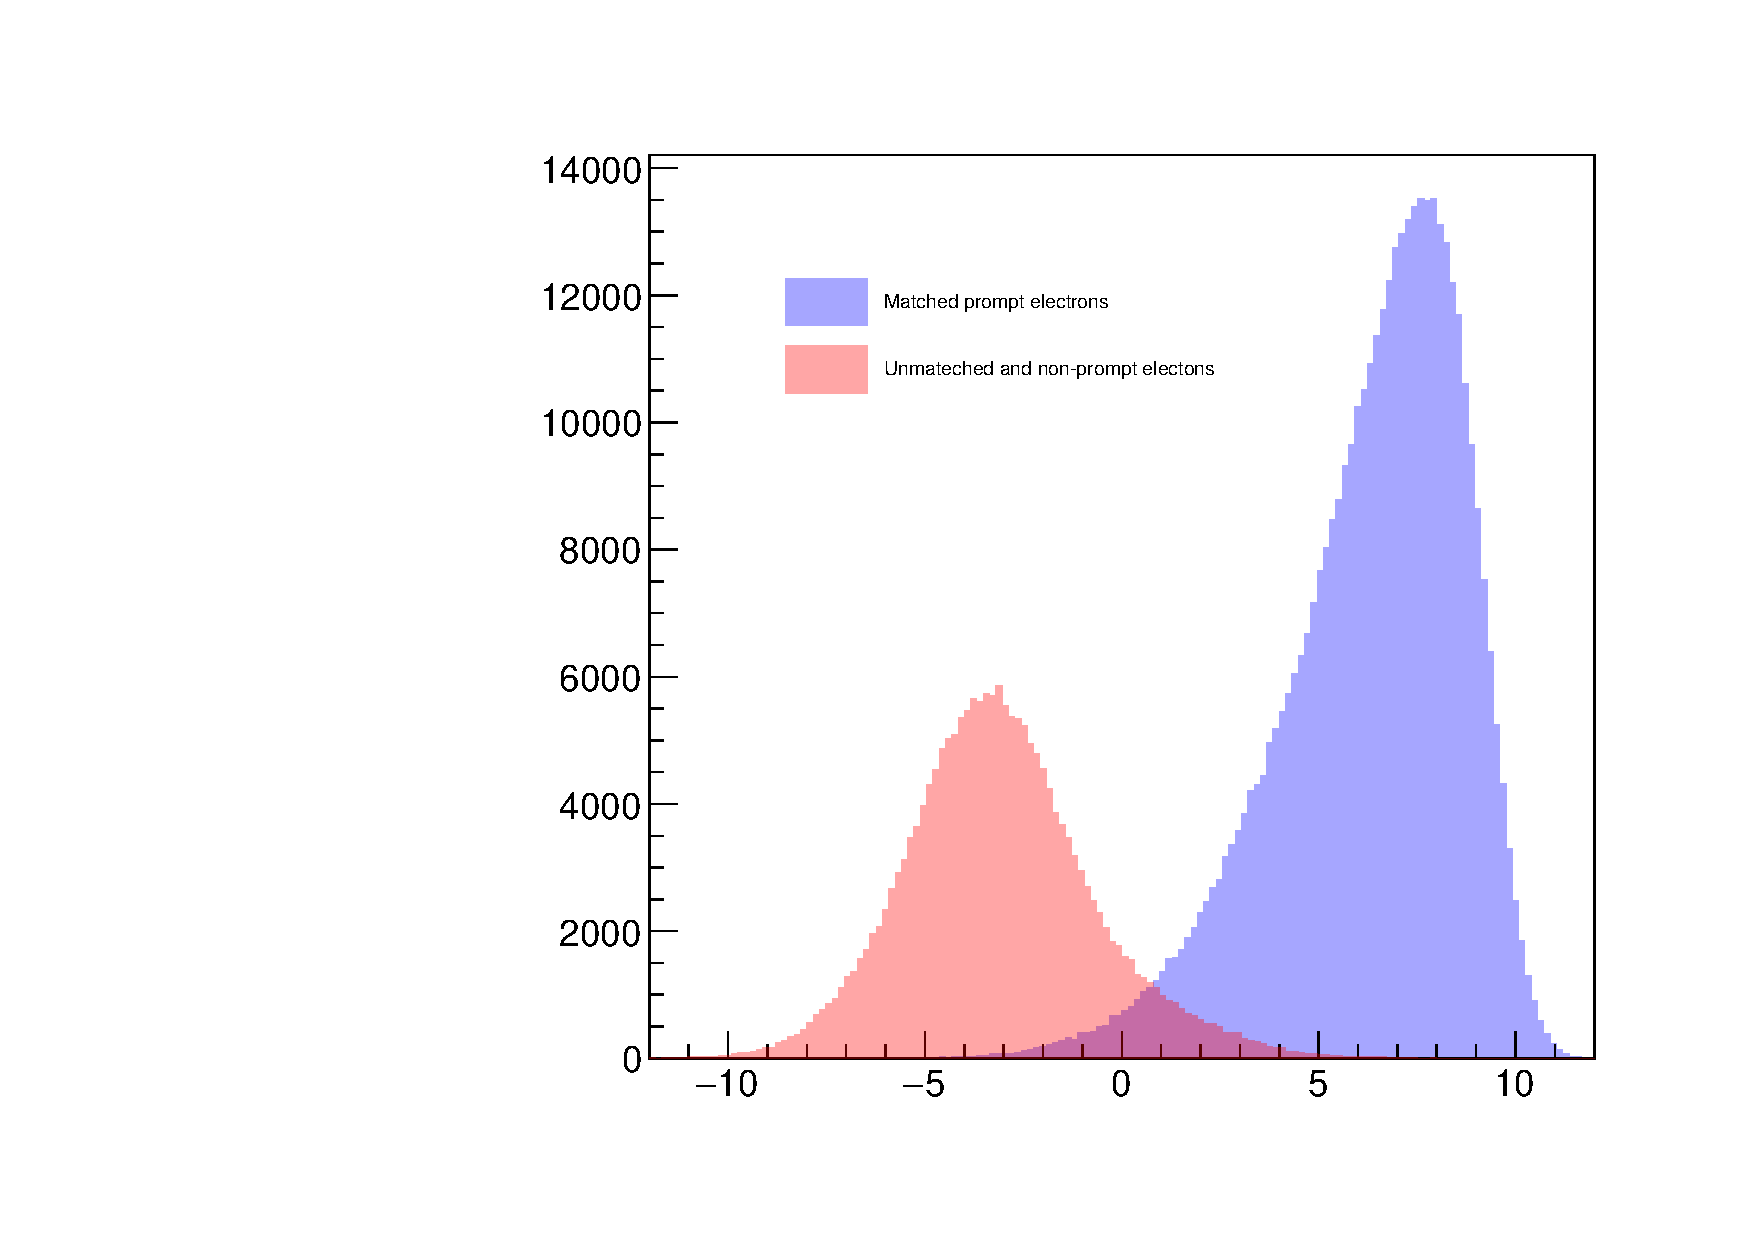
\includegraphics[width=0.80\textwidth]{Figures/Electrons/Ele_BDTv2_Score.pdf}
\caption{Output of the multiclassifier discriminant for prompt electrons matched to truth electrons from Z decay (blue) and for fakes (red). Events are all taken from DY events MC sample.
\label{fig:ele_ID_output}}
\end{center}
\end{figure}

The impact of the transition from the TMVA(v1) to the xgboost(v2) training library is shown in Fig.~\ref{fig:ele_ID_ROC}.
The working points shown are chosen so as to get the  same signal efficiency as a cut on MVA ID and a cut on the PF isolation, in each $p_T$ and $\eta$ bin.

\begin{figure}[!htb]
\vspace*{0.3cm}
\begin{center}
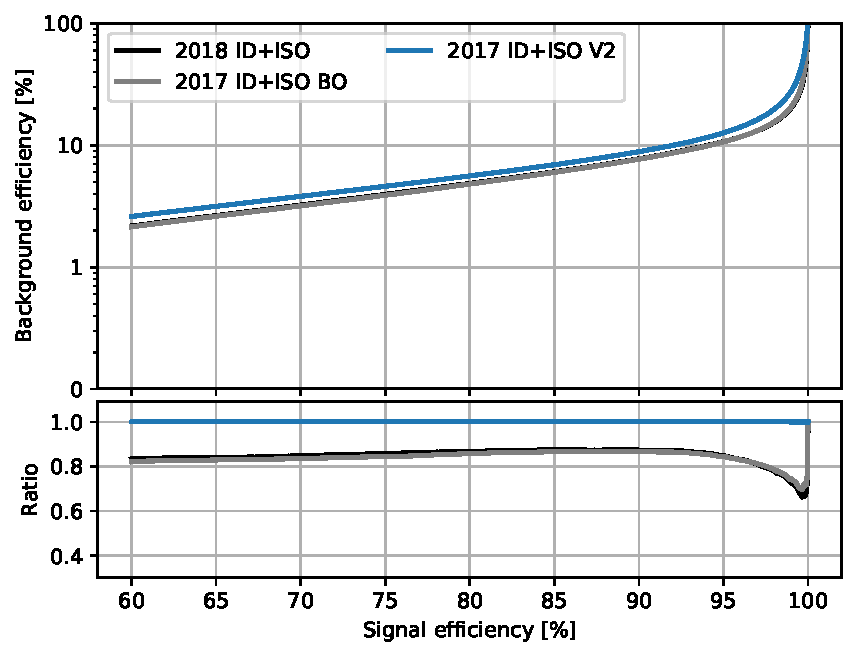
\includegraphics[width=0.45\textwidth]{Figures/Electrons/2018_EB1_5.pdf}
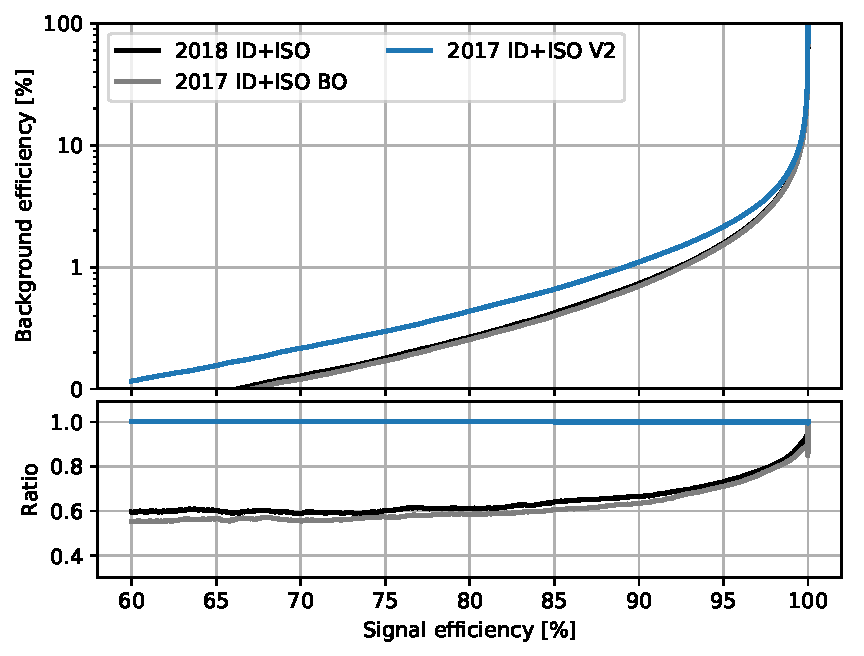
\includegraphics[width=0.45\textwidth]{Figures/Electrons/2018_EB1_10.pdf} \\
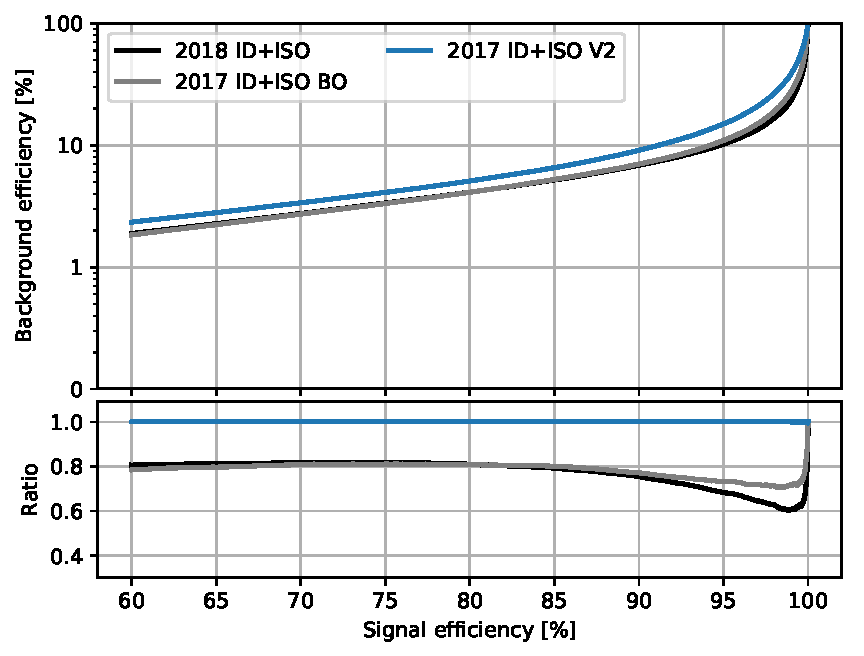
\includegraphics[width=0.45\textwidth]{Figures/Electrons/2018_EB2_5.pdf}
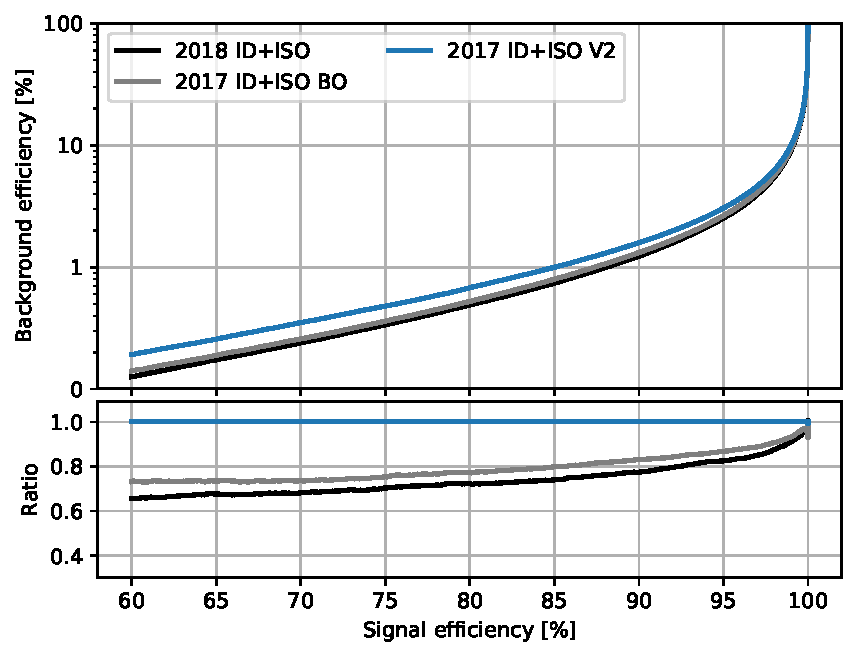
\includegraphics[width=0.45\textwidth]{Figures/Electrons/2018_EB2_10.pdf} \\
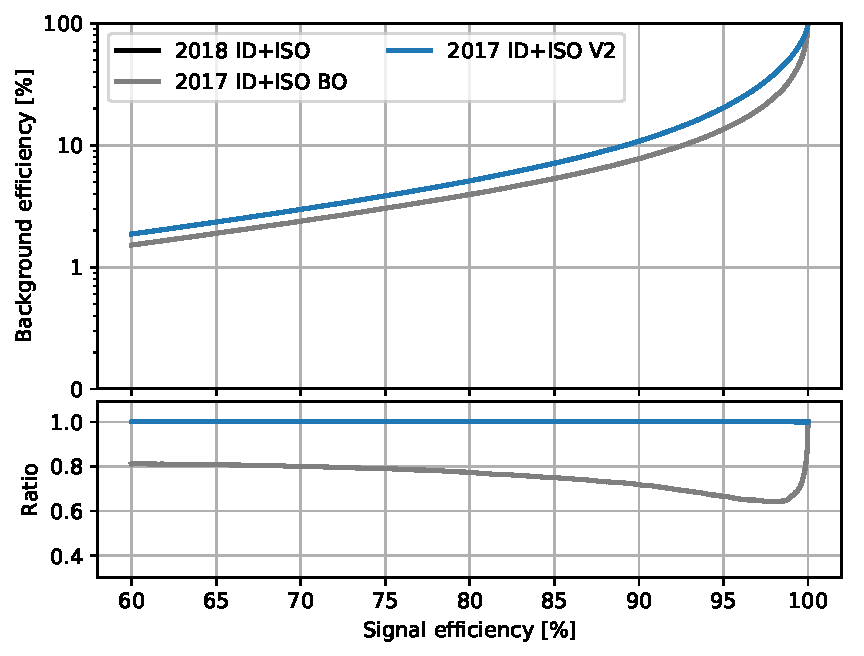
\includegraphics[width=0.45\textwidth]{Figures/Electrons/2018_EE_5.pdf}
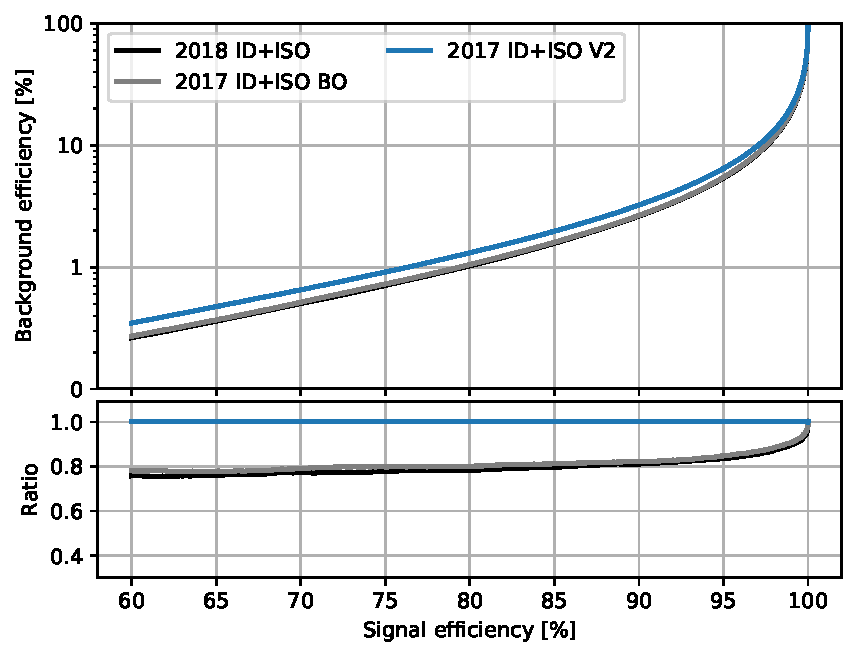
\includegraphics[width=0.45\textwidth]{Figures/Electrons/2018_EE_10.pdf} \\
% \caption{Performance comparison (background efficiency vs signal efficiency) of the MVA's trained for the 2017 analysis combining identification and isolation (black), 2016 training MVA ID + cut on PF isolation (blue) and 2017 training MVA ID + cut on PF isolation (orange). Dots are working points chosen for this analysis. The 2017 working point is chosen to have the same signal efficiency as 2016 analysis. Performance are shown for electrons with $5 < p_T < 10 $~GeV (left), $p_T > 10 GeV$~(right) and $|\eta|<0.8$~(top), $0.8 < |#eta| < 1.479$~(middle) and $|#eta| > 1.479$~(bottom).
\caption{The receiver operating characteristic curves (background efficiency vs signal efficiency) of the MVA's trained on the 2017 simulation and applied on the 2018 simulation. The training combines identification and isolation variables. Performance are shown for electrons with $5 < p_T < 10 $~GeV (left), $p_T > 10 GeV$~(right) and $|\eta|<0.8$~(top), $0.8 < |#eta| < 1.479$~(middle) and $|#eta| > 1.479$~(bottom). V1 and V2 versions of training are compared, exploiting TMVA and xgboost training libraries respectively.
\label{fig:ele_ID_ROC}}
\end{center}
\end{figure}

% The BDT was finally re-retrained with the last version of the MC (Fall17 v2). The difference between the two trainings, as shown in the Fig~\ref{fig:ele_ID_ROCv2}, is small. All the final results shown later in this document are done with v1 version, but we will switch to the v2 version together with the implementation of latest scale/smearing corrections, scale factors provided by the POGs, etc...
%
%
% \begin{figure}[!htb]
% \vspace*{0.3cm}
% \begin{center}
% \includegraphics[width=0.45\textwidth]{Figures/Electrons/2017_EB1_5.pdf}
% \includegraphics[width=0.45\textwidth]{Figures/Electrons/2017_EB1_10.pdf} \\
% \includegraphics[width=0.45\textwidth]{Figures/Electrons/2017_EB2_5.pdf}
% \includegraphics[width=0.45\textwidth]{Figures/Electrons/2017_EB2_10.pdf} \\
% \includegraphics[width=0.45\textwidth]{Figures/Electrons/2017_EE_5.pdf}
% \includegraphics[width=0.45\textwidth]{Figures/Electrons/2017_EE_10.pdf} \\
% %\caption{Performance comparison (fakes per event vs signal efficiency) of the MVA's trained for the 2017 analysis with (orange) and without (blue) isolation as input variables, without isolation in the BDT but as cuts (green), as well as 2016 MVA with 2016 PU conditions (black) or re-weighted to 2017 PU conditions (dotted black line).This plot is for electrons in the barrel only.
% \caption{Performance comparison (background efficiency vs signal efficiency) of the MVA's trained for the 2017 analysis combining identification and isolation for v1 (blue) and v2 (orange) MC training (blue). Ratio between v1 or v2 training wrt a training on 2016 MC is also shown in the bottom. Dots are working points chosen for this analysis. The 2017 working point is chosen to have the same signal efficiency as 2016 analysis. Performance are shown for electrons with $5 < p_T < 10 $~GeV (left), $p_T > 10 GeV$~(right) and $|\eta|<0.8$~(top), $0.8 < |#eta| < 1.479$~(middle) and $|#eta| > 1.479$~(bottom).
% %The respective working points are indicated by the markers.
% \label{fig:ele_ID_ROCv2}}
% \end{center}
% \end{figure}



% \begin{figure}[!htb]
% \vspace*{0.3cm}
% \begin{center}
% \includegraphics[width=0.5\textwidth]{Figures/Electrons/ele_overtraining.png}
% \caption{BDT output for the training and testing sample for true and fake electrons in the high-$p_T$ endcap training bins.
% \label{fig:ele_ID_BDT_output}}
% \end{center}
% \end{figure}

%Table~\ref{tab:ele_ID_input_variables} summarizes the full list of observables used as input to the classifier
Table~\ref{tab:ele_ID_WP} lists the cut values applied to the BDT score for the chosen working point.
For the analysis, loose electrons have to pass this MVA identification and isolation working point.

%\begin{table}[h!]
%\scriptsize
%    \centering
%    \begin{tabular}{c|c c c}
%\multicolumn{4}{|c|}{Datasets}                                                                 \\
%\hline %----------------------------------------------------------------------------------------
%minimum BDT score    &  $|\eta| < 0.8 $ & $0.8 < |\eta| < 1.479$ 	& $|\eta| > 1.479$      \\
%\hline %----------------------------------------------------------------------------------------
%$ 5 < p_T < 10 $ GeV &  1.264      & 1.178  		& 1.330		\\
%$p_T > 10$ GeV       &  2.364		& 2.078		&  1.080		\\
%\hline %----------------------------------------------------------------------------------------
%\hline %----------------------------------------------------------------------------------------
%     \end{tabular}
%\small
%    \caption{Minimum BDT score required for passing the electron identification.}% \textbf{FIXME: WP to be defined!}}
%    \label{tab:ele_ID_WP}
%\end{table}


%2016
 = (pt<=10 && ((fSCeta<0.8                  && BDT >  0.95034841889) ||
                                   (fSCeta>=0.8 && fSCeta<1.479 && BDT >  0.94606270058) ||
                                   (fSCeta>=1.479               && BDT >  0.93872558098)))
                    || (pt>10  && ((fSCeta<0.8                  && BDT >  0.3782357877) ||
                                   (fSCeta>=0.8 && fSCeta<1.479 && BDT >  0.35871320305) ||
                                   (fSCeta>=1.479               && BDT >  -0.57451499543)));

%2017
   isBDT         = (pt<=10 && ((fSCeta<0.8                  && BDT >  0.85216885148) ||
                                   (fSCeta>=0.8 && fSCeta<1.479 && BDT >  0.82684550976) ||
                                   (fSCeta>=1.479               && BDT >  0.86937630022)))
                    || (pt>10  && ((fSCeta<0.8                  && BDT >  0.98248928759) ||
                                   (fSCeta>=0.8 && fSCeta<1.479 && BDT >  0.96919224579) ||
                                   (fSCeta>=1.479               && BDT >  0.79349796445)));


\begin{table}[h!]
\scriptsize
    \centering
    \begin{tabular}{|c|c c c}
%\multicolumn{4}{|c|}{Datasets}                                                                 \\
%\hline %----------------------------------------------------------------------------------------
\cline{2-4}
  \multicolumn{1}{ c|}{}             & \multicolumn{3}{|c|}{$|\eta| < 0.8 $}                        \\                      
\cline{2-4} %----------------------------------------------------------------------------------------
   \multicolumn{1}{c|}{}            & Cut on BDT score & Signal eff. & \multicolumn{1}{c|}{Background eff.}  \\ 
\hline %----------------------------------------------------------------------------------------
$ 5 < p_T < 10 $ GeV              & 1.264                        & 81.04\%            &  \multicolumn{1}{c|}{4.4\%}  \\                   
\hline %----------------------------------------------------------------------------------------
 $p_T > 10$ GeV                     &  2.364		& 97.1\%		&  \multicolumn{1}{c|}{2.9\%}		\\
\hline %----------------------------------------------------------------------------------------
\cline{2-4}
  \multicolumn{1}{ c|}{}             & \multicolumn{3}{|c|}{$0.8 < |\eta| < 1.479$}                        \\            
\cline{2-4} %----------------------------------------------------------------------------------------
   \multicolumn{1}{c|}{}            & Cut on BDT score & Signal eff.      & \multicolumn{1}{c|}{Background eff.}  \\
\hline  %----------------------------------------------------------------------------------------
$ 5 < p_T < 10 $ GeV              & 1.178                     & 79.3\%           &  \multicolumn{1}{c|}{4.6\%}     \\
\hline %----------------------------------------------------------------------------------------
$p_T > 10$ GeV                      &  2.078		         & 96.3\%	  &  \multicolumn{1}{c|}{3.6\%}		\\
\hline %----------------------------------------------------------------------------------------

\cline{2-4}
  \multicolumn{1}{ c|}{}             & \multicolumn{3}{|c|}{$|\eta| > 1.479$}                        \\            
\cline{2-4} %----------------------------------------------------------------------------------------
   \multicolumn{1}{c|}{}            & Cut on BDT score & Signal eff. & \multicolumn{1}{c|}{Background eff.}  \\
\hline  %----------------------------------------------------------------------------------------
$ 5 < p_T < 10 $ GeV              & 1.330                     & 72.97\%    &  \multicolumn{1}{c|}{3.6\%}     \\
\hline %----------------------------------------------------------------------------------------
$p_T > 10$ GeV                      &  1.080		         & 95.7\%      &  \multicolumn{1}{c|}{6.7\%}		\\
\hline %----------------------------------------------------------------------------------------

     \end{tabular}
\small
    \caption{Minimum BDT score required for passing the electron identification, together with the corresponding signal and background efficiencies, for 2018 samples..}% \textbf{FIXME: WP to be defined!}}
    \label{tab:ele_ID_WP}
\end{table}


